\section{Opis systemu STOS}
\indent System Testowania i~Oceny zadań Studenckich (w skrócie „STOS”), to system dedykowany dla prowadzących zajęcia na Politechnice Gdańskiej. Umożliwia testowanie rozwiązań stworzonych przez studentów podczas zajęć projektowych oraz laboratoryjnych, pod kątem wydajności i~poprawności. Przepływ pracy polega na przesłaniu kodu programu przez studenta do systemu, kompilacji po stronie serwera oraz przesłaniu wyniku na podstawie serii testów zdefiniowanych przez prowadzącego.

\section{Komponenty i~schemat działania}
System możemy podzielić na komponenty ze względu na realizowane zadania:
\begin{itemize}
    \item STOS-ui -- serwis w~postaci strony internetowej, umożliwiający wgranie rozwiązań przez studentów i~umieszczenie ich w~kolejce dostępnej do pobrania przez inne serwisy poprzez żądania HTTP. Oprócz kolejki posiada również bazę danych z ocenami prac studentów. Serwis posiada warstwę prezentacji, która generuje przyjazne dla użytkownika widoki.
    \item Moduł sprawdzający -- część serwisu działającego po stronie serwera. Jego zadaniem, jest wywoływanie zapytań do API udostępnianego przez serwis STOS-ui metodą odpytywania, w~celu pobierania kodu programów do wykonania, zlecenie kompilacji, ocenę kodu oraz przesłanie wyniku do STOS-u.
    \item Moduł kompilujący -- skonteneryzowany serwis działający na serwerze, kompilujący otrzymany kod. Ma możliwość kompilacji lub interpretacji wielu języków programowania. Aktywnie nasłuchuje komunikatów przesyłanych przez nazwany potok. Jest przystosowany do ciągłego działania, co wymaga uruchomienia go wyłącznie przy starcie całej platformy. Posiada współdzielone katalogi z~gospodarzem, zawierające skrypty kontrolujące, kody źródłowe oraz rezultaty.
\end{itemize}
\begin{figure}
	\begin{center}
		\resizebox{1.0\textwidth}{!} {
			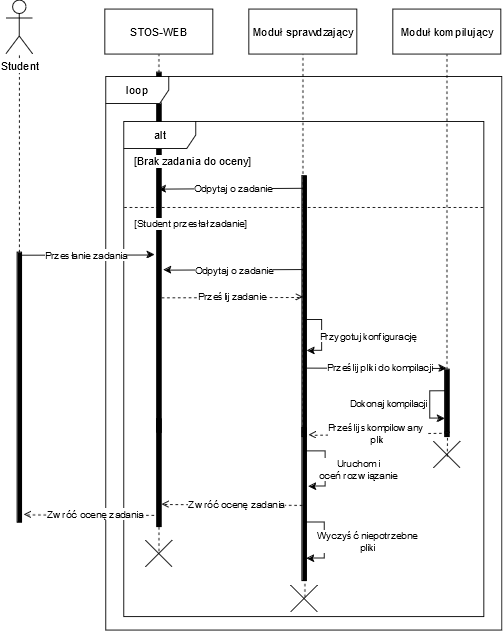
\includegraphics{img/1/d_sek_1.png}
		}
		\caption[Diagram sekwencji komponentów]{Diagram przedstawiający sekwencję wykonywanych zdarzeń w~systemie, podczas oceny zadania. Źródło własne.}
	\end{center}
\end{figure}

\section{Proces uruchamiania}
Przed uruchomieniem systemu, należy zwrócić uwagę na konfigurację użytkowników oraz struktury katalogowej. Pliki uruchamianego systemu muszą być umieszczone w~katalogu \textit{/home/stos}, ze względu na niemodyfikowalne bez zmiany skryptów ustawienie ścieżek. Należy upewnić się, czy istnieją wszyscy użytkownicy, którzy są wymienieni w~skryptach, czyli „ja” oraz „stos”, oraz pozostałe skrypty i~pliki wykonywalne, używane w~trakcie działania modułów.
\newline \indent Uruchamianie platformy na docelowym serwerze odbywa się poprzez użycie dwóch skryptów:
\begin{itemize}
    \item start.sh -- uruchamianie kontenera kompilującego zadania.
    \item startup.sh -- uruchamianie serwisu pobierającego, przekazującego i~sprawdzającego zadania przesłane przez studentów.
\end{itemize}
Skrypt startup.sh pobiera adres VPN z interfejsu sieciowego \textit{tap1}. 

\section{Uproszczona struktura katalogowa}
\dirtree{%
.1 root.
.2 io-result.php.
.2 qapi.
.3 qctrl.php.
.2 stos.
.3 common-final.sh.
.3 fsapi.
.3 get.sh.
.3 handle-vc.sh.
.3 get.sh.
.3 judge.exe.
.3 qapi.
.3 runscript.
.3 sendresult.
.3 serve.sh.
.3 setup.sh.
.3 start.sh.
.3 startup.sh.
.3 stop.sh.
.3 sync.sh.
.3 vs-compile.sh.
.3 vc-final.sh.
.3 control.
.4 base.sh.
.4 regwine.reg.
.4 run.sh.
.4 vs.sh.
.4 vcbase.sh.
.3 io.
.4 result/.
.4 src/.
.4 input.
.4 output.
}
W zaprezentowanej strukturze katalogowej, ze względu na powtarzalność i~identyczność działania, nie zostały uwzględnione pliki kompilujące inne języki niż C lub C++. Pliki z folderu \textit{io}, służą do komunikacji z modułem kompilującym, a~skrypty z katalogu \textit{control}, są używane do jego sterowania. Część z plików jest w~postaci binarnej, przystosowanych do uruchomienia w~systemie Linux albo Windows.